\documentclass[10pt,twocolumn]{article}
\usepackage{graphicx}
\usepackage{amssymb}
\usepackage{titling}
\usepackage{tabularx}
\usepackage{url,hyperref}
\pagenumbering{gobble}
\begin{document}

\title{Classifying post-secondary school funding type based on student debt and
earnings}

\author{Shay Lehmann and Michelle Ho}

\date{%
CUSP-GX-5006\\
Prof. Gustavo Nonato\\
Machine Learning Assignment \# 3\\
\rule{\textwidth}{1pt}
}

\posttitle{\par\rule{3in}{0.4pt}\end{center}\vskip 0.5em}
%\postdate{\rule{\textwidth}{1pt}}

\maketitle

\begin{abstract}
In this assignment, the authors explore how 4-year colleges in the United States
can be classified into funding types (public, private for-profit, or private non-profit) based
on data on the debt and earning outcomes of their students.
The exercise aims to compare Support Vector Machines (SVM), decision trees (CART),
and Random Forests (with and without boosting) as
classification techniques and their in performance in a real life scenario.
\end{abstract}

\section{Introduction}
The main goals of this assignment are to compare three classification techniques and
to better understand how earning and debt outcomes of students vary by the types
post-secondary institutions they attend. The motivation is to ultimately understand
what indicates a "high value" education for the final project of this course.

The dataset used in this assignment is provided by the U.S. Department
of Education project, College Scorecard. The goal of the project is to provide data
necessary for students and their families to compare and assess
post-secondary institutions on their costs and student outcomes. The data is
compiled from self-reported data from institutions, data on federal financial aid, and
tax information for the past 20 years. This rich dataset
includes measurements on multiple aspects of a postsecondary institution-- including basic
identifying information, admissions, student body demographics, degree programs,
tuition costs, federal aid, debt repayment, completion rates, and earnings.

Our hope is that students and their families who are making decisions on
post-secondary education can make use of our results to compare schools.
Institutions themselves can use the results to assess how their students perform
compared to peer institutions. Finally, loan granting institutions and the U.S.
Department of Education can assess which schools are failing in preparing their
students for career success and why.

\section{Methods and Data Sets}

In order to have data on earnings and repayment outcomes after graduation,
this assignment uses only the 2010 - 2011 College Scorecard, since wage and debt data is not yet
available for the years after 2011. This dataset contains
7414 institutions and 1743 variables. However, there is not complete coverage for
all variables depending on the institution. For this assignment, subsets of the raw
dataset was used for analysis, and the variables and data cleaning steps are
described below:

\begin{itemize}
\item \texttt{CONTROL}: a categorical variable indicating the funding type of a school.
Categories are 1=``public", 2=``private non-profit", or 3=``private for-profit".
\item \texttt{REGION}: a categorical variable indicating the region of the United States
where the school is located. Regions are:
\begin{itemize}
\item New England (CT, ME, MA, NH, RI, VT)
\item Mid East (DE, DC, MD, NJ, NY, PA)
\item Great Lakes (IL, IN, MI, OH, WI)
\item Plains (IA, KS, MN, MO, NE, ND, SD)
\item Southeast (AL, AR, FL, GA, KY, LA, MS, NC, SC, TN, VA, WV)
\item Southwest (AZ, NM, OK, TX)
\item Rocky Mountains (CO, ID, MT, UT, WY)
\item Far West (AK, CA, HI, NV, OR, WA)
\item Outlying Areas (AS, FM, GU, MH, MP, PR, PW, VI)
\end{itemize}
\item \texttt{GRAD\char`_DEBT\char`_MDN}: Median debt for students who graduate
\item \texttt{WDRAW\char`_DEBT\char`_MDN}: Median debt of students who withdrew without completion
\item \texttt{GRAD\char`_DEBT\char`_MDN10YR}: Median debt by monthly payment (10 year plan) for graduates
\item \texttt{MN\char`_EARN\char`_WNE\char`_P7}: Mean earnings of students working and not enrolled 7 years
after entry
\item \texttt{COMPL\char`_RPY\char`_3YR\char`_RT\char`_SUPP}: 3-year repayment rate for students who completed degrees,
suppressed for institutions of fewer than 30 students
\item \texttt{NONCOM\char`_RPY\char`_3YR\char`_RT\char`_SUPP}: 3-year repayment rate for students who did not
complete degrees, suppressed for institutions of fewer than 30 students
\item \texttt{LO\char`_INC\char`_DEBT\char`_MDN}: The median debt for students with family income between \$0-\$30,000
\item \texttt{HI\char`_INC\char`_DEBT\char`_MDN}: The median debt for students with family income \$75,001+
\item \texttt{MD\char`_INC\char`_DEBT\char`_MDN}: The median debt for students with family income between \$30,001-\$75,000
\item \texttt{LOAN\char`_EVER}: Share of students who received a federal loan while in school
\item The dependent variable being classified and predicted is `Control' in this assignment's
analyses. The authors may occasionally refer to this variable as `Y'.
\item The independent variables are all the others.
\item Only institutions classified as \texttt{ICLEVEL = 1} (eg. 4-year colleges) are used.
\item Any observations with null values for any of the chosen variables
are dropped. After these drops, the number of observations
in the dataset is 2249 and 2433 for the two subsets used. The breakdown school types
represented in the second subset is in Table 1, and was similar for the first subset.
There were more private non-profit schools than private for-profit and public schools
in the dataset.
\item Finally, the categorical variable \texttt{REGION} is binarized so that all samples
are represented by boolean feature vectors.
\end{itemize}

The steps taken for this assignment:

\begin{enumerate}
\item A classification model is fitted for selected independent variables with
a SVM Linear model (Model 1) at varying training sizes
\item Next, a second SVM linear classification model is fitted using a second subset
of independent variables (Model 2) with training size of 70\% of the dataset
\item Next, decision tree classifier models are fitted on the second subset of independent variables
      with varying depths of tree allowed. The training size of all trees is set at 70\%.
\item Next, decision tree classifier models are done without boosting (Model 3), with bagging (Model 4),
with ADA boosting (Model 5), and with gradient boosting (Model 6) at varying depths.
\item All models are assessed via cross validation on training and test sets split
from the original dataset. The training and test set sizes are adjusted to assess the effect of training size on quality
of classification.
\item Confusion matrices and a plot of in-sample and out-sample errors
are created for all models of the dependent variable
``Control" to assess the performance of the classifications
\end{enumerate}

\section{Results}

The first classification model was SVM with a linear kernel, fitted on the variables:\\
\texttt{REGION},\\
\texttt{GRAD\char`_DEBT\char`_MDN},\\
\texttt{WDRAW\char`_DEBT\char`_MDN},\\
\texttt{GRAD\char`_DEBT\char`_MDN10YR},\\
\texttt{MN\char`_EARN\char`_WNE\char`_P7},\\
\texttt{COMPL\char`_RPY\char`_3YR\char`_RT\char`_SUPP}, and\\
\texttt{NONCOM\char`_RPY\char`_3YR\char`_RT\char`_SUPP}.\\

The dataset was split into
training sets of 20\%, 40\%, 60\%, and 80\% of the whole. The performance
was not very good, and misclassified approximately 50 percent of the data for all
training sizes (See Table 2). The confusion matrix with training size 80\% can be found
in Figure 1.

To focus on loan and debt variables, a second smaller subset of variables is chosen only
for debt and loan variables:\\

\texttt{LO\char`_INC\char`_DEBT\char`_MDN},\\
\texttt{HI\char`_INC\char`_DEBT\char`_MDN},\\
\texttt{MD\char`_INC\char`_DEBT\char`_MDN}, and\\
\texttt{LOAN\char`_EVER}.\\

Model 2, like Model 1, is a linear SVM classification model.
The confusion matrix for the model fitted with 70\% of training data can be found
in Figure 2. Similarly, this model does not perform especially well outside of the
the training set.

We find that decision tree classifier models in general performed better than
support vector machines in classifying school types based on debt and earnings data.
A regular decision tree model set with increasing tree depths (Model 3)
shows that the in-sample error quickly approaches zero (see Figure 3).
However, out-sample error does not see much improvement. The decision tree does
very well in separating within the training dataset, but it does not do as well
with the test data. However, with additional bagging of varying base estimator sizes (Model 4),
the problem of overfitting appears to improve. In fact, the out of sample error
rate decreases from about 25\% to 20\%, when comparing decision tree
classification without bagging and with bagging at different depths (see Figure 4).

We see a similar improvement with Model 5 (decision tree with ADA boosting), Model 6
(decision tree with gradient boosting) and
Model 6 (random forest classifier). The increase of base estimators appear to have
the greatest improvement on both in-sample and out-of-sample error when the tree
maximum depth is small. In our examples, this is when it is set to 5. Figures 5 - 7
are line plots of the errors from Models 5 - 7 with varying parameter sizes.

\section{Conclusions}

In summary, we demonstrate that classification with decision trees
were able to perform better than SVM on predicting school funding types
with this particular dataset. Furthermore, decision trees can be improved
with additional boosting and bagging techniques, with improvements
depending on the maximum depth of the tree.

Further steps of this assignment would be to vary the training sizes to assess
performance, and then possibly add in years of data prior to 2010 to increase size.

Python code used to generate the results, tables, and figures for this assignment can be
found at \url{https://github.com/michellemho/machine_learning_for_cities}.


\begin{table*}[ht]
\centering
\caption{Percentages of each school type represented in dataset (second subset)}
\label{my-label}
\begin{tabular}{lllll}
& Type                & Percentage &\\
& Public              & 27.08            & \\
& Private Non-Profit  & 45.05    & \\
& Private For-profit  & 27.87  & \\
                &                           &
\end{tabular}
\end{table*}

\begin{table}[ht]
\caption{Percentage of Misclassification, Model 1} % title of Table
\centering % used for centering table
\begin{tabularx}{\columnwidth}{c c c} % centered columns (4 columns)
\hline
Training Size Percent & In-Sample Error & Out-Sample Error \\ [0.5ex] % inserts table
%heading
\hline % inserts single horizontal line
20 & 49.88 & 52.56 \\ % inserting body of the table
40 & 49.27 & 54.0 \\
60 & 48.85 & 55.0 \\
80 & 49.03 & 51.11 \\ [1ex] % [1ex] adds vertical space
\hline %inserts single line
\end{tabularx}
\label{table:model1}
\end{table}

\begin{figure*}[!t]
  \begin{center}
    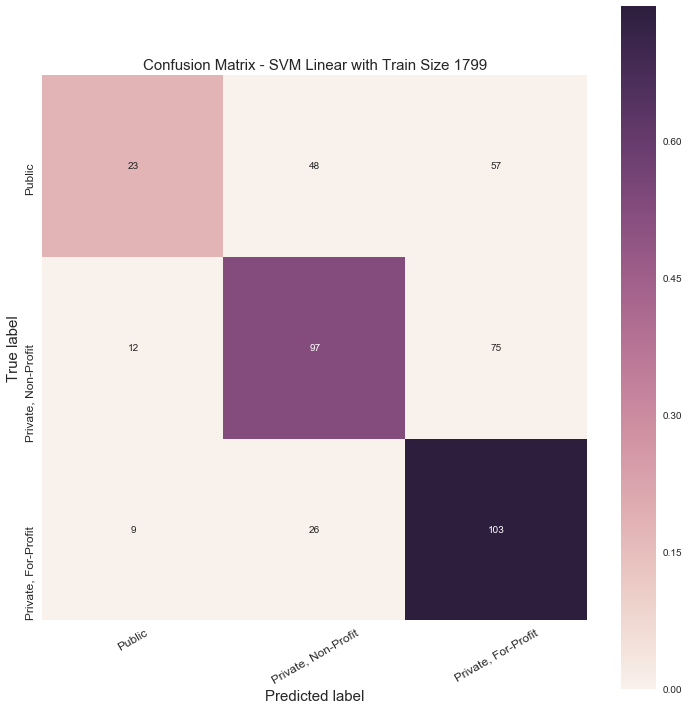
\includegraphics[width=6in]{MODEL1_80trainsize.png}
  \end{center}

  \caption{\small Model 1 Confusion Matrix}
  \label{fig-1}
\end{figure*}

\begin{figure*}[!t]
  \begin{center}
    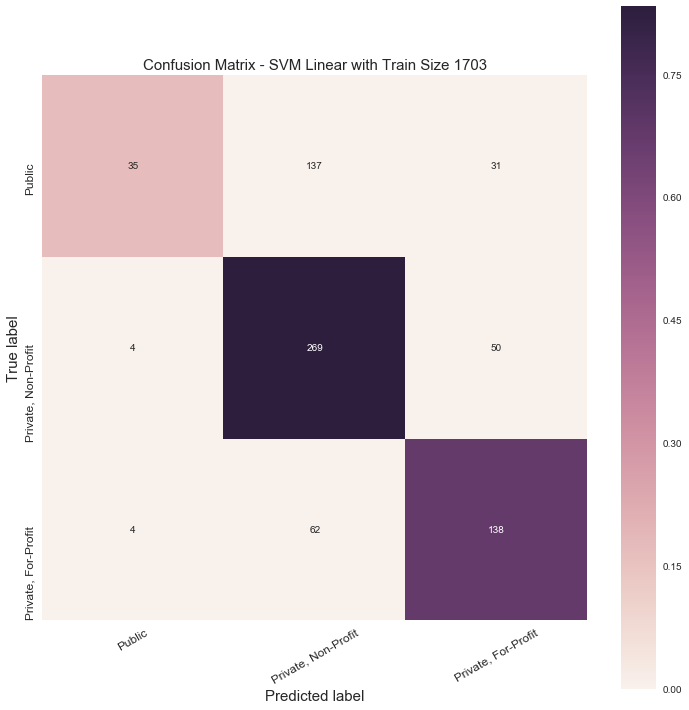
\includegraphics[width=6in]{MODEL2_trainsize70.png}
  \end{center}

  \caption{\small Model 2 Confusion Matrix}
  \label{fig-1}
\end{figure*}

\begin{figure*}[!t]
  \begin{center}
    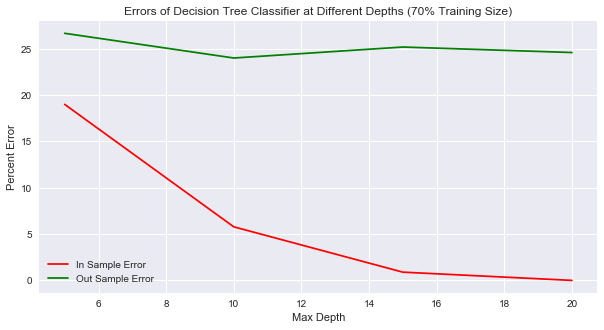
\includegraphics[width=\textwidth,height=\textheight,keepaspectratio]{decision_tree_error_1.png}
  \end{center}

  \caption{\small Model 3}
  \label{fig-1}
\end{figure*}

\begin{figure*}[!t]
  \begin{center}
    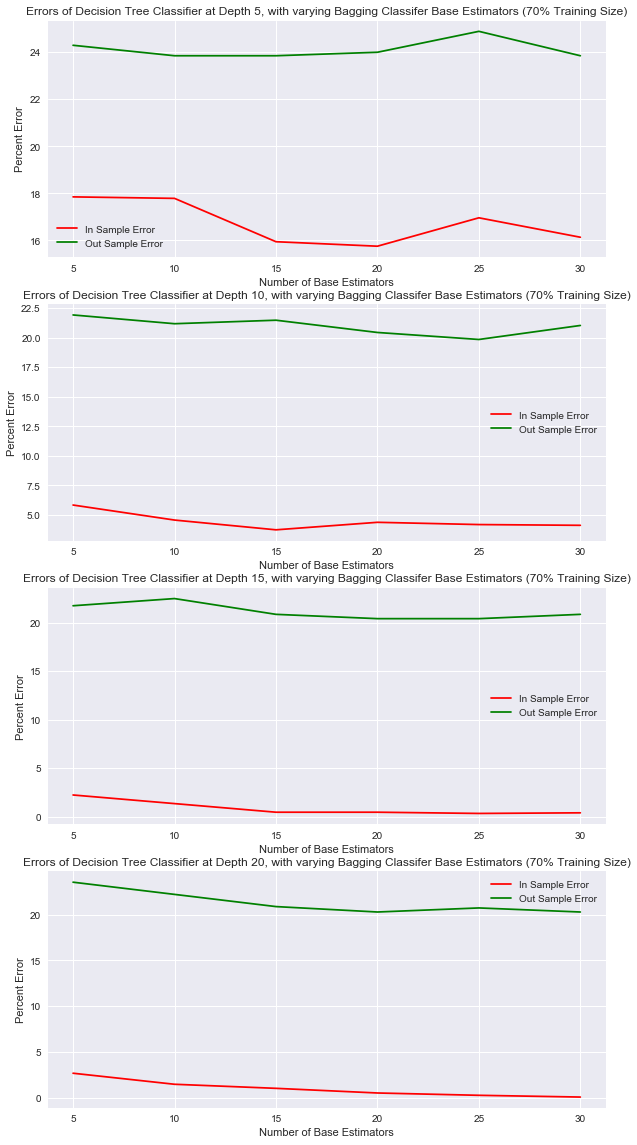
\includegraphics[width=\textwidth,height=\textheight,keepaspectratio]{decision_tree_bagging.png}
  \end{center}

  \caption{\small Model 4}
  \label{fig-1}
\end{figure*}

\begin{figure*}[!t]
  \begin{center}
    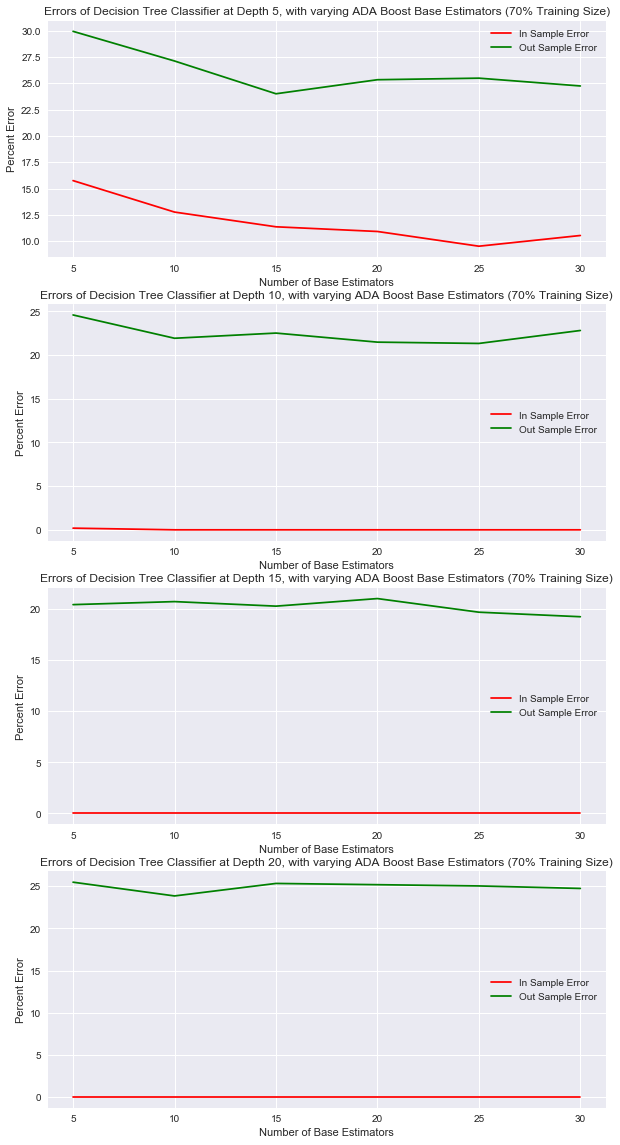
\includegraphics[width=\textwidth,height=\textheight,keepaspectratio]{ada_boost.png}
  \end{center}

  \caption{\small Model 5}
  \label{fig-1}
\end{figure*}

\begin{figure*}[!t]
  \begin{center}
    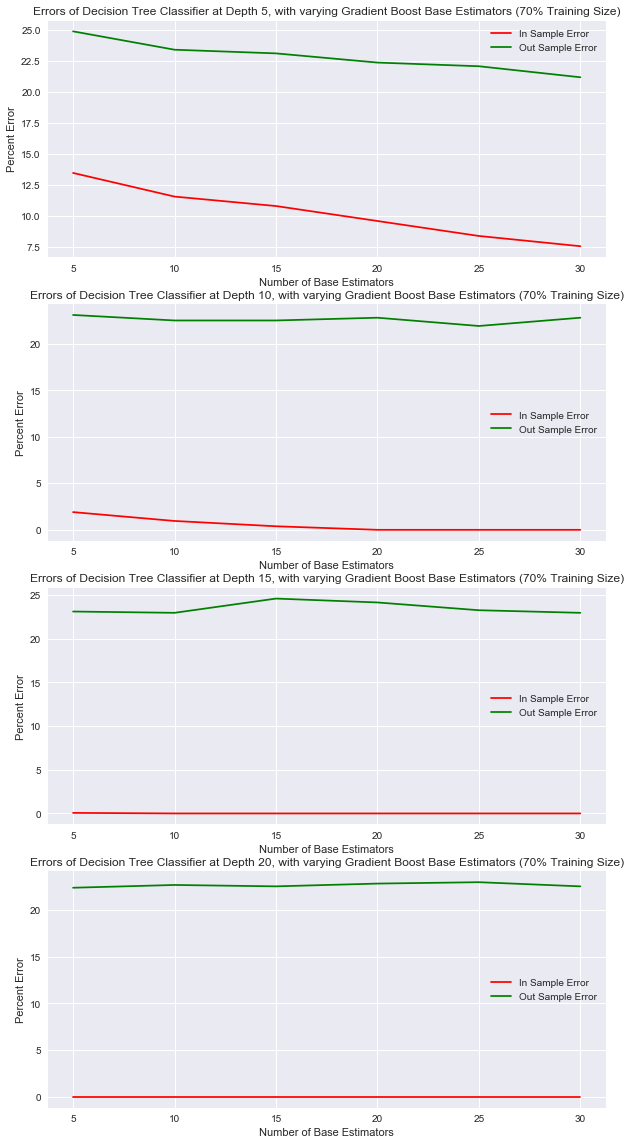
\includegraphics[width=\textwidth,height=\textheight,keepaspectratio]{gradient_boost.png}
  \end{center}

  \caption{\small Model 6}
  \label{fig-1}
\end{figure*}

\begin{figure*}[!t]
  \begin{center}
    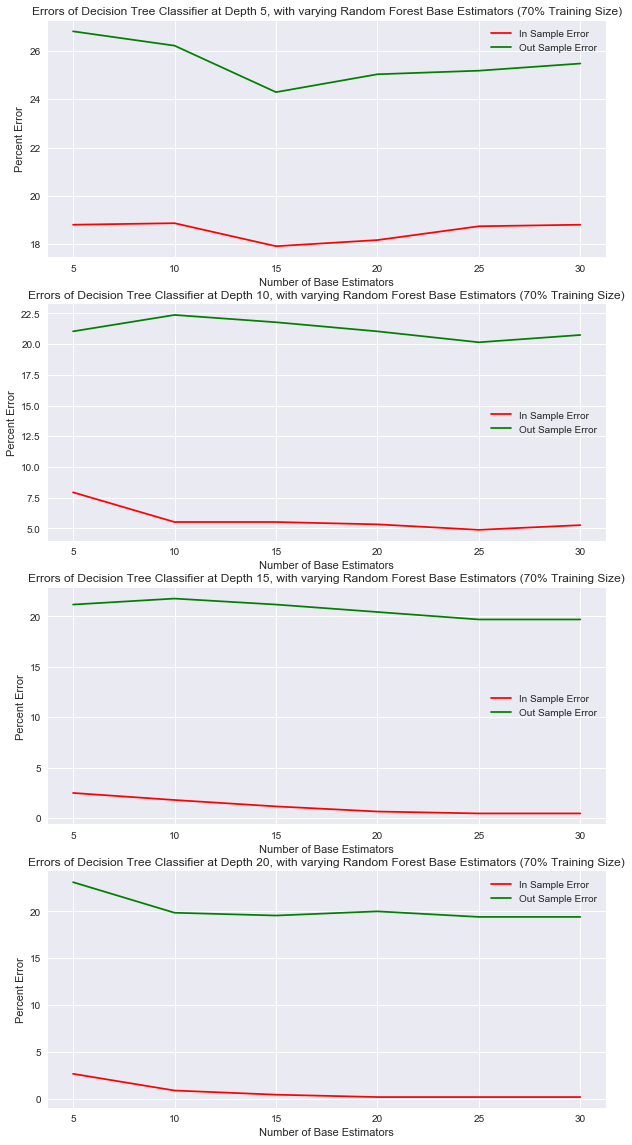
\includegraphics[width=\textwidth,height=\textheight,keepaspectratio]{randomforest.png}
  \end{center}

  \caption{\small Model 7}
  \label{fig-1}
\end{figure*}

\end{document}
